\documentclass[12 pt]{article}
\usepackage{amsfonts}
\usepackage{amsmath,amsthm,amssymb}
\usepackage{graphicx}
\usepackage{hyperref}
\usepackage{cancel}
\usepackage[english]{babel}
\usepackage{blindtext}
\usepackage{color}
\usepackage{multicol}
\usepackage{units}
\usepackage{siunitx}
\usepackage{tocbibind}
\usepackage{subcaption}
\usepackage{caption}

\setlength{\textheight}{9.5in}
\setlength{\textwidth}{6.5in}
\setlength{\topmargin}{-0.5in}
\setlength{\oddsidemargin}{0in}
\setlength{\evensidemargin}{0.75in}
\setlength{\parskip}{0.15in}
\setlength{\parindent}{0in}
\usepackage[utf8]{inputenc}
\usepackage[T1]{fontenc}
\usepackage{longtable}

\usepackage[usenames,dvipsnames]{xcolor}  %%%this package is required for latex code in svg graphics

\usepackage{titlesec}
\titlespacing*{\chapter}{0pt}{-50pt}{20pt}
\titleformat{\chapter}[display]{\normalfont\huge\bfseries}{\chaptertitlename\ \thechapter}{20pt}{\Huge}


\begin{document}

%%Title Page %%%%%%%%%%%%%%
\begin{titlepage}
\centering

	\vspace{1cm}
	{\scshape\Large Mathematics Extended Essay\par}
	\vspace{3cm}
	{\huge\bfseries Patterns in the Cut Loci of House-Shaped Polyhedra\par}
	\vfill

% Bottom of the page
	{\large \today\par}
\end{titlepage}

\tableofcontents
%\listoffigures

\newpage
\graphicspath{ {Images/} }

%%%%%%%%%%%%%%%%%%%Abstract Start %%%%%%%%%%%%%%%%%%%%
\section*{Abstract}

This essay examines how unfolding algorithms, which are algorithms that decompose 3D polyhedra into 2D planar nets, unfolds polyhedra whose shape resembles a house. These polyhedra are strictly defined to be all polyhedra that can be composed of a regular, right prism and a regular pyramid which have congruent bases. The results of the algorithm are then analyzed to produce a conclusion about the following research question, which is inspired by an open problem posed by Aronov and O'Rourke\cite{ROURKE}: Does the cut locus of a polyhedron approach its medial axis as the number of lateral faces the polyhedron increases and approaches a smooth surface?

The algorithm being used is the Star Unfolding algorithm, first developed by Alexandrov. The algorithm uses cuts on the surface of a convex polyhedron to define the edges of the unfolded planar net of the polyhedron, and then continuously unfolds it into a planar net. The cuts are defined by determining a minimum spanning tree from an arbitrary source point, from which every node defines at least two vertices of the unfolded planar net and each edge defines two edges. 

A cut locus is then defined as the Voronoi edges of the vertices of the UPN. We define the cut loci for 10 cases of house-shaped polyhedra, and then prove a conclusion.

\textbf{Word Count:} 216

\newpage

%%%%%%%%%%%%%%%%%%%%%%Introduction
\section{Introduction}
In recent years computational origami has garnered much attention for the exploration of computer science applications within origami, an art form about cutting and folding paper into various shapes. One of the most notable applied science achievements the field has produced were algorithms to determine a method for folding and compacting large, rigid objects into small spaces for later deployment. These algorithms have seen extensive uses in space technology industries, such as in 1996, when Koryu Miura deployed the solar arrays of a Japanese satellite by unfolding it in outer space \cite{FOLDIT:1}.
In addition to having algorithms for folding 3D shapes, there also exist algorithms to create unfoldings of a polyhedron, that is to say decompose it into a flat, planar net. For example, the net of a cube would be considered an unfolding of a polyhedra:
%Cube Figure
\begin{figure}[h]
\caption{Example unfolding of a cube. Taken from O'Rourke (2011)}
\centering
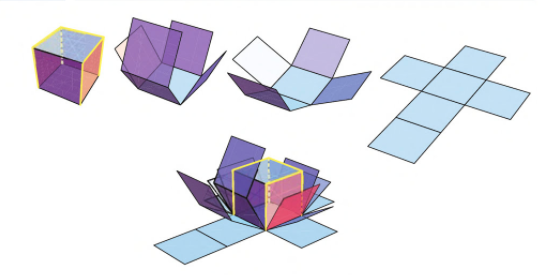
\includegraphics[scale=0.5]{latinCross.png}
\end{figure}

Unfolding is generally made by defining a series of cuts along the surface of a polyhedron, and then mapping the edges and vertices of the cuts onto a plane. In the cube example, cuts are first made along the edges and then the cube is "opened up" into the planar net. Since the cuts are only made along the edges, this kind of unfolding is called an edge unfolding.

There exists another kind of unfolding, called general unfolding, which allows any kind of cutting to be made on the surface of polyhedra and which Demaine et al have proven to work for all polyhedra of a certain type.\cite{GFALOP:1} In this essay, I will examining how the cut locus of the output of a general unfolding algorithm called the "star unfolding" changes for a series of polyhedra as they approach a curved shape. This research topic offers another perspective on an open problem posed by Aronov and O'Rourke (1992):

$$\mbox{Prove or disprove whether or not the cut locus approaches the medial axis of the house-shaped polyhedra as the number of lateral sides increase and as they approach a smooth surface.}$$

These developments in unfolding may ultimately lead to further insights into more efficient designs for shelters.

	Before heading into the analysis, I will first be establishing the definitions of what we are trying to find, as well as the keywords needed to reach the goal.

\section{Definitions}

%%Citation Test
\subsection*{House-Shaped Polyhedra}
House-shaped polyhedra are defined as the set, $H$, of composite shapes embedded within $\mathbb{R}^3$ made by joining an $n$-sided, right, regular prism to a regular, $n$-sided base pyramid by the bases. Individual polyhedra are referred to as $H_n$, where the value of $n$  begins at 3, since a prism base of $n=2$ would not yield a shape in $\mathbb{R}^3$. The bases where the pyramid and prism join are removed to leave just the outside geometry. The lateral faces of the house-shaped polyhedra are also defined as being the lateral faces of both the pyramid and the prism, where the number of lateral faces is also denoted by n.

\begin{figure}[h]
\caption{$H_3$}
\centering
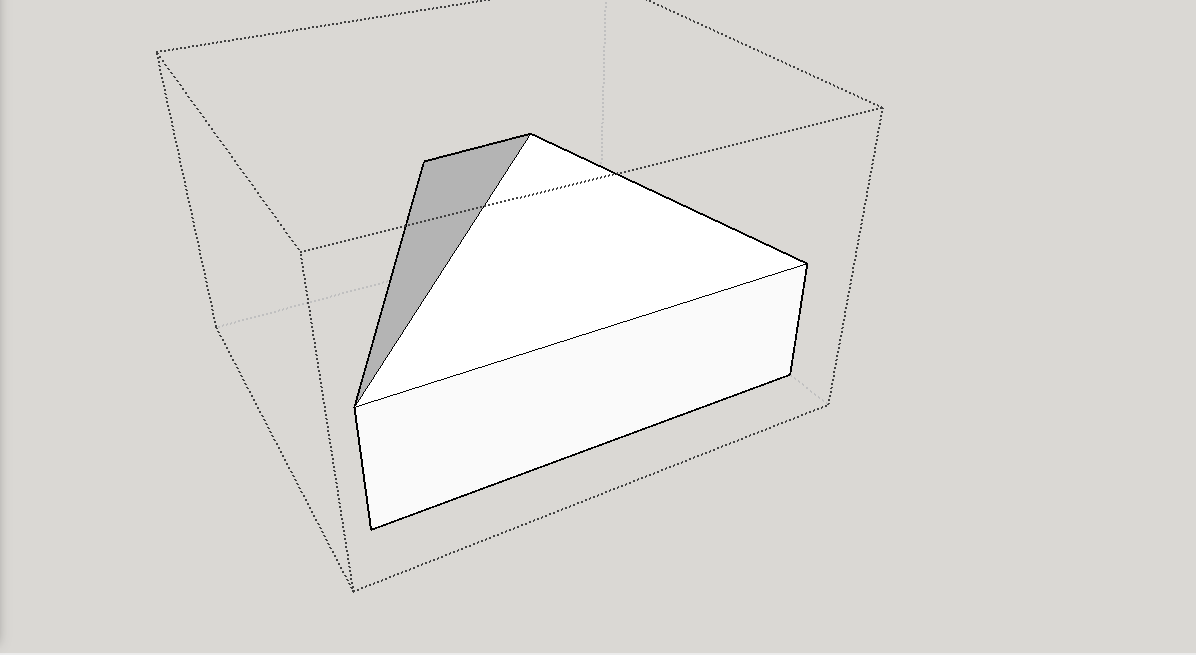
\includegraphics[scale=0.15]{starUnfolding/h3.png}
\end{figure}
\begin{figure}[h]
\caption{$H_4$}
\centering
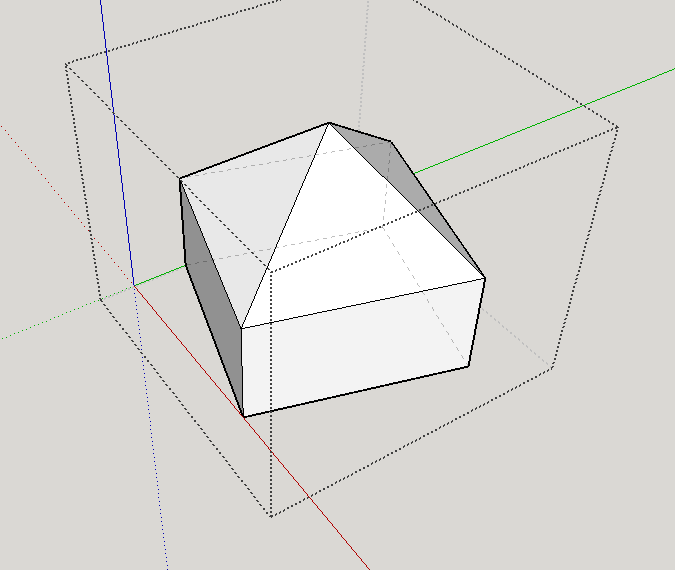
\includegraphics[scale=0.15]{starUnfolding/h4.png}
\end{figure}

\begin{figure}[h]
\caption{$H_7$}
\centering
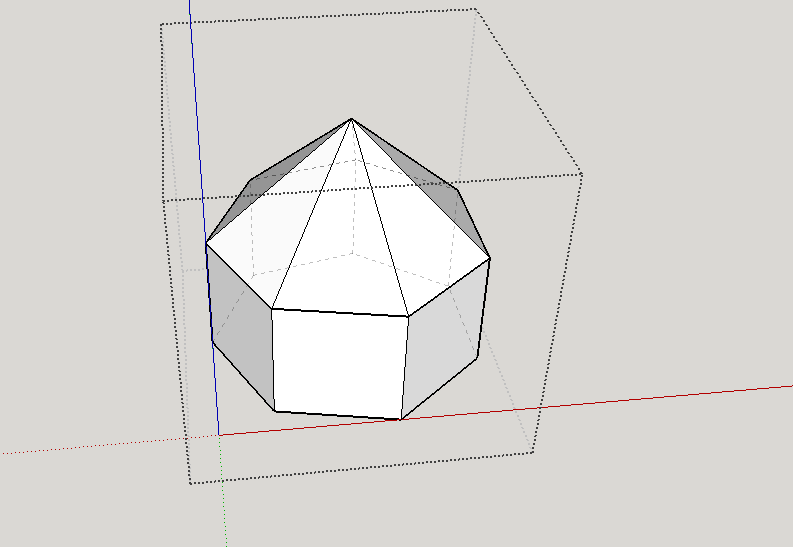
\includegraphics[scale=0.15]{starUnfolding/h7.png}
\end{figure}

\subsection*{Medial Axis}
The medial axis of a shape in $\mathbb{R}^2$ is the the set of all points that share at least 2 distinct shortest paths from the boundary of the shape.\cite{GFALOP:1}

\begin{figure}[h]
\caption{Medial Axis of a rectangle.\cite{MEDAX}}
\centering
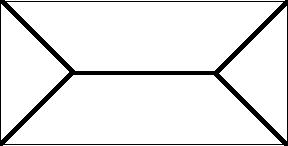
\includegraphics[scale=0.45]{medax.jpg}
\end{figure}

\subsection*{Voronoi Diagrams}
	Let $S$ be a set of points on a plane $F$. A Voronoi diagram is defined as the partitioning of plane $F$ into regions where every point in the region is the closest point to a point in $S$ using Euclidean distance .\cite{GFALOP:1} The points that are equidistant from two points in $S$ form a Voronoi edge, which define the boundaries for each region .\cite{GFALOP:1}
\begin{figure}[h]
\caption{Example of a Voronoi Diagram. Taken from Wikimedia under CC licensing.}
\centering
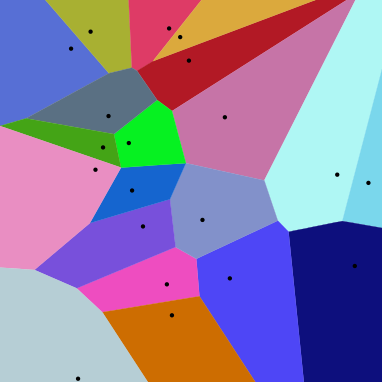
\includegraphics[scale=0.5]{voronoi.png}
\end{figure}
\subsection*{Cut Locus}
	The cut locus is the set of Voronoi edges that are produced from drawing a Voronoi diagram using the vertices of the unfolded planar net generated from a star unfolding.\cite{GFALOP:1} This definition has some similarities with the idea of a medial axis because it is defined also by the points which have at least 2 shortest lengths leading to them. The open problem posed by Aronov and O'Rourke (1992) is the following:
	"Prove or disprove the conjecture that the cut locus for a point $x$ on a smooth convex surface develops (without overlap) to the medial axis of the boundary of the star unfolding, which is composed of the images of the source $x$."

\subsection*{Unfolded Planar net (UPN)}
An unfolded planar net (UPN) is a polygon that is generated from applying general unfolding algorithms to a polyhedron. They are defined from a tree of cuts on the surface of the polyhedron which splits its faces and introduces extra edges onto the surface. After the faces are split, the UPN can be defined by unfolding the polyhedron such that every edge of the cutting tree defines 2 edges and every node defines 2 vertices of a polygon in $\mathbb{R}^2$.

\subsection*{Cutting Tree}

	Going back to how we unfolded the cube in the introduction, remember that we had to make a few cuts along the edges of the cube so that we may unfold it. That series of cuts can be obtained by defining a cutting tree for the cube. For general unfoldings, we can also define cutting trees that are not restricted to just the edges of a polyhedron and that may split the faces of a polyhedron.
	
Defining a cutting tree requires several definitions beforehand of the concepts of graph theory which underlie it. Call a collection of $V$ vertices and $E$ edges, which connect the vertices a \textbf{graph}, $G(V,E)$. A graph which has the edges connecting a set of ordered vertices $v_1, v_2, v_3, ...v_i$ is called a \textbf{directed graph}. If $v_a$ is connected to $v_b$, then the two vertices are adjacent, which is denoted as $v_a \textasciitilde v_b$. Let $C$ be a directed graph with vertices $v_1, v_2, v_3, ...v_i$ be connected in such a way that satisfies the condition $\forall i \in 1,2,3,... i-1, \ v_i \textasciitilde v_{i+1}$. Call $C$ a \textbf{walk}. A \textbf{path} is a walk where each vertex is only connected to two other vertices, or in other words, $v_i \neq v_j, \forall i \neq j$. A graph is \textbf{connected} if there exists a path between each of its vertices. A \textbf{tree} is a connected graph with no cycles , meaning that the path doesn't loop back on itself and $v_1\neq v_i$. \cite{STANFORD}

Let $p$ be a polyhedron embedded in $\mathbb{R}^3$. A cutting tree is defined as a tree on the polyhedral surface $P$ of $p$ that produces a valid unfolding within an algorithm. 

The cutting tree for a star unfolding is defined as the minimum spanning tree is a tree on the surface $P$ of a polyhedron starting from a source point $x$ that touches all vertices of the polyhedron based on the shortest distance travelled across $P$ [citation needed]. In the context of this essay, the definition of cutting tree for a star unfolding will be the one that is used.
\subsection*{Star Unfolding}

A Star Unfolding of a polyhedron $p$ produces a UPN based upon a cut tree $T$ on the surface $P$ of $p$. It is guaranteed to work for convex polyhedra [citation needed]. 

The Star Unfolding algorithm is a general unfolding algorithm developed by Alexandrov (Durer?). Demaine et al have proven that it works for any convex polyhedron, and we will be using it to construct several unfoldings so as to analyze their cut loci.

\subsection*{Gaussian Curvature}
When you run your hand along an object, sometimes the surface will feel curved and your hand will either curl inwards or bend backwards as it traces the surface. The concept of curvature is used to describe how that object curve away or towards your hand, and it is used often in differential geometry for the study of smooth and curved surfaces.

Curvature will be used in this essay to describe the surfaces of polyhedra, specifically using the angle deficit definition of curvature developed by Gauss[citation needed. Also footnote for Descartes]. Let point $a$ be an angle on polyhedral surface $P$. Gaussian curvature of a polyhedra, referred to as ?the curvature? from now on, is defined as 2$\pi$ minus the sum of incident face angles at $a$.
For example, the curvature at one of the corners (Figure \ref{cubeAngles}) of a cube is: 
$$360-3(\ang{90}) = \ang{90}$$
$$\mbox{or:}$$
$$2\pi - 3(\pi/4) = \pi/4$$

\begin{figure}[h]
\caption{The incident face angles of a cube's vertex.}
\centering
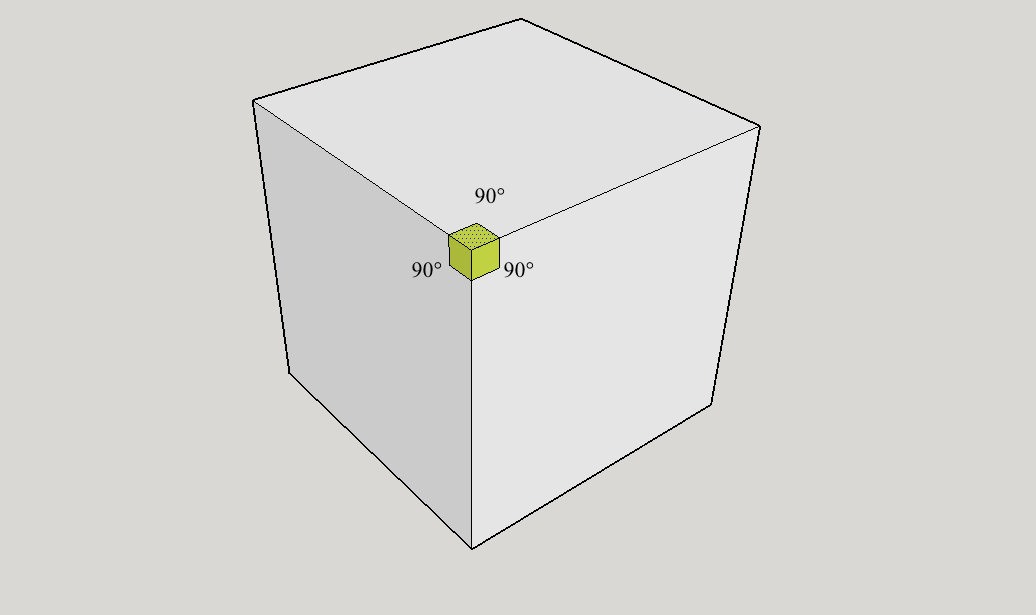
\includegraphics[scale=0.35]{cubeCurvature.png}
\label{cubeAngles}
\end{figure}

	The sign of final result indicates whether or not the curvature is positive or negative. If a polyhedron has a dip in its shape, the vertices within that dip will have the angles formed by their adjoining edges add up to greater than 360 degrees, leading to a negative curvature once the sum is subtracted from 360. 
	
(Negative Curvature Diagram)
Taken from Demaine (2007)

	Note that the only points of the curvature on flat surface polyhedra are at the vertices.

\subsection*{Convex Polyhedron}
	A convex polyhedron is a polyhedra that is has only positive curvature on its vertices. Demaine et al have proven that all convex polyhedra can have an UPN which can be obtained through a general unfolding algorithm. Since we are trying to locate a pattern within the series of house-shaped polyhedra, we need to make sure that all polyhedra within $H$ are convex.

\section{Convexity of House-Shaped Polyhedra}
	Before we begin applying the star unfolding algorithm on house-shaped polyhedra, I'm going to make sure that no cases of non-convexity appear in house-shaped polyhedra as sides are added. This is to say cases of negative curvature doesn't come up as n increases to infinity.
	
	The statement to be proven is that there is never be a case where a house-shaped polyhedron becomes non-convex as we increase the number of lateral sides on the house shaped polyhedra. Star unfoldings of every house-shaped polyhedra would then be guaranteed.
	
Since house-shaped polyhedra are made from right, regular prisms and regular pyramids, they possess rotational symmetry. This means that we only need to check that curvature will always be positive for the 2 distinct vertices which border a lateral side of the prism (Fig.4).

\begin{figure}[h]
\caption{Bottom: $v_1$ Top: $v_2$}
\centering
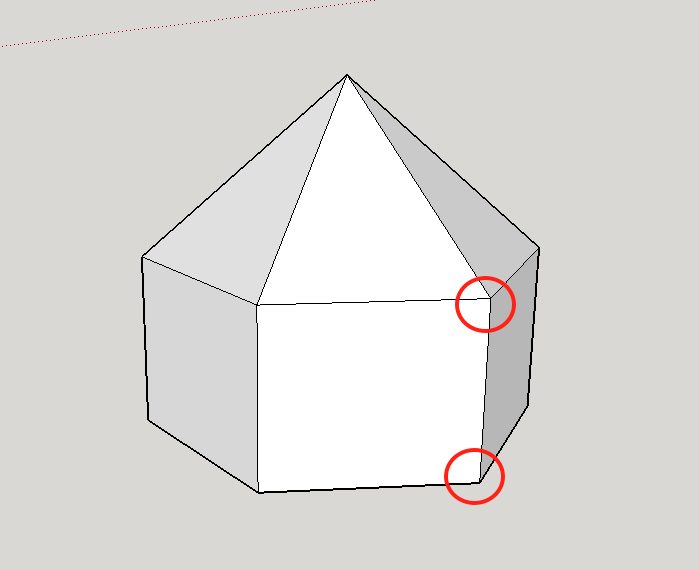
\includegraphics[scale=0.35]{rotSymmetry.png}
\end{figure}

The apex of the pyramid must have positive curvature since it is at the height of the pyramid.

Call the bottom vertex on the base of the prism $v_1$ and the vertex between the pyramid and the prism $v_2$. $v_1$ lies on 2 edges that are a part of the prism's base and 1 edge that's a part of the lateral side. Since the prism is a right prism, the incident face angles of the lateral side are \ang{90}. The incident face angle formed by the edges on the base, however, are determined by the internal angle of the regular polygon that forms the base. 
The internal angle of regular polygons is determined by the formula \cite{ANGLES}:

$$\theta_i = \cfrac{180(n-2)}{n}$$
Where $n$ is the number of sides on the regular polygon. 
Going back to house-shaped polyhedra, curvature at a vertex becomes negative once the sum of the adjoining angles is greater than \ang{360}. Since $v_1$ already has$v_1$ 2 adjoining angles of \ang{360}, the curvature at these vertices will remain positive so long as the internal angle of the base does not exceed \ang{360}. 
Taking the limit of n to positive infinity of the equation shows us that this is indeed true:

$$\lim_{n\to+\infty} \cfrac{180(n-2)}{n} =  \lim_{n\to+\infty}\cfrac{180n-360}{n} = \lim_{n\to+\infty}\cfrac{n\left(180-\frac{360}{n}\right)}{n} =  \lim_{n\to+\infty}\left(180-\frac{360}{n}\right) = 180$$

As additional lateral sides are added to the polyhedron, the internal angle of the base will approach \ang{180}. However, this value will never exceed \ang{180}, therefore the curvature at $v_1$ will always remain positive.

The internal angle does however equal \ang{360} at $n=+\infty$, resulting in a curvature of 0. 

%%%%Needs editing. Consider the new definition for curvature.
However, because we can only consider cases of house-shaped polyhedra with discrete values of n, this can never happen to any individual house-shaped polyhedra within the series. In other words,  $v_1$ always have a positive curvature because it doesn't make sense to have a polygonal base with infinite sides.

	As for the top vertices, the angles formed by the lateral edge of the pyramid are slightly rotated and elevated above what would have been the top of the regular prism. It is easy to prove, however, that these angles must be strictly less than \ang{360}, because for the top of the house-shaped polyhedron to be a regular pyramid, the lateral sides of the top must be triangles. Therefore, the angles must be less than \ang{360}, since triangles in Euclidean geometry have angles which sum to \ang{360}, and by extension, the curvature of the vertices must be positive. 
	
\section{Cutting Tree}
Before we can define the star unfolding of a polyhedron $H_n$, we need to first define the cutting tree for $H_n$ from which we can map out an UNP. Let $T$ represent a tree on the polyhedral surface $P$ of $H_n$. A cutting tree is defined as the minimum spanning tree starting from an arbitrary source point $x\in P$. \cite{GFALOP:1}

For the ease of drawing minimum spanning trees and to compare the unfoldings of different house-shaped polyhedra, I chose the source point to be a point very close to the circumcentre of the bases of each polyhedra. The reason for this is to avoid having multiple shortest paths branching from the source point to the vertex at the top of the pyramid, which would affect the definition of the cutting tree.

\begin{figure}[h]
\caption{$H_3$ minimum spanning tree from $x$ (unseen)}
\centering
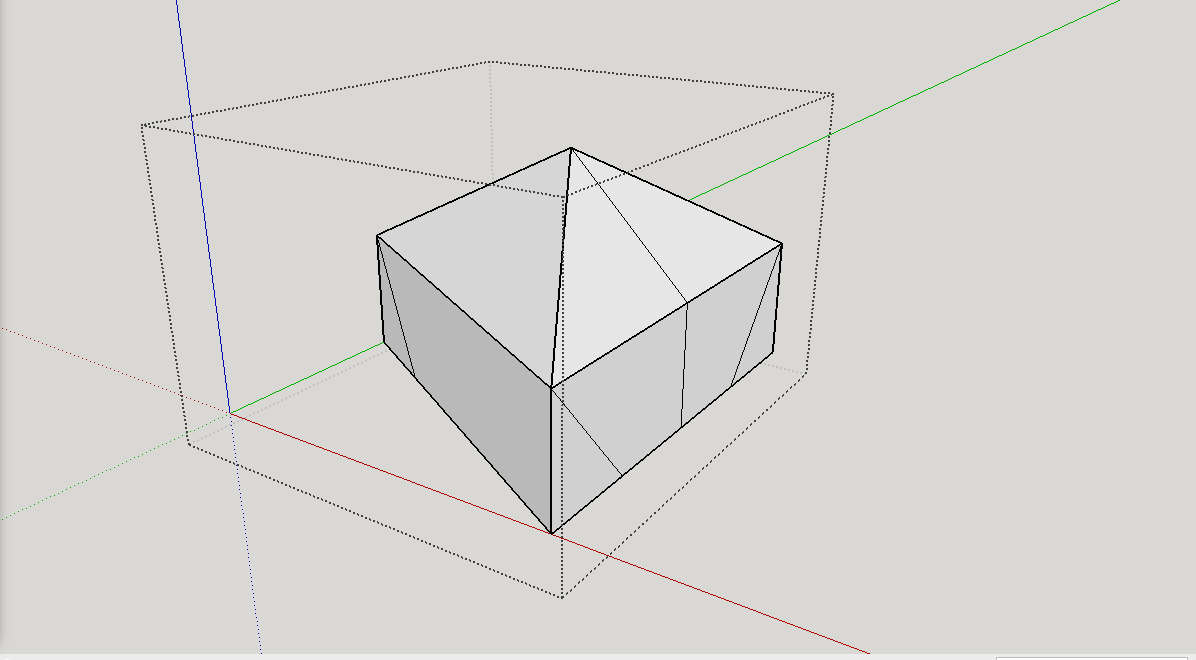
\includegraphics[scale=0.35]{starUnfolding/h3FinalIso.png}
\end{figure}

To find the minimum spanning tree, I turned to finding the geodesics of the polyhedra which connect $x$ and the vertices of $H_n$ to define a shortest path.

A geodesic is a curve $\Gamma$ on a polyhedral surface $P$ between two points $x$ and $y$ that is locally minimized \cite{GFALOP:1}, that is to say, it appears as a straight line when walking along the surface of the polyhedron. For example, longitude lines along the Earth are geodesics, but lattitude lines are not, because they require a traveller along the path to turn in order to stay on the line. 

The reason geodesics are useful in this situation is because of their property to locally minimise distances, which can be used to define spanning trees. Furthermore, geodesics appear as straight lines on the surface of polyhedra. As such, straight lines can be drawn from $x$ to each vertex across the surface of a polyhedron to define a minimum spanning tree.

These straight lines can be drawn on an edge unfolding of the polyhedron. The edge unfolding is a way of making the polyhedral surface flat, which is how it would look from the perspective of the geodesic. The polyhedron can then be refolded to yield the spanning tree.
For cases $n=\{3,4,5,6,50\}$, I  used Google Sketchup to determine their cutting trees and to illustrate them in diagrams.
Although I've made the height of the pyramids in the diagram equal to the height of the prism, all diagrams involving house-shaped polyhedra don't have to be to scale. Star unfoldings and their cutting trees for other house-shaped polyhedra with different height ratios can still exist.

\begin{figure}[h]
\caption{$H_3$ edge unfolded and with shortest paths drawn on the base. $x$ is circled.}
\centering
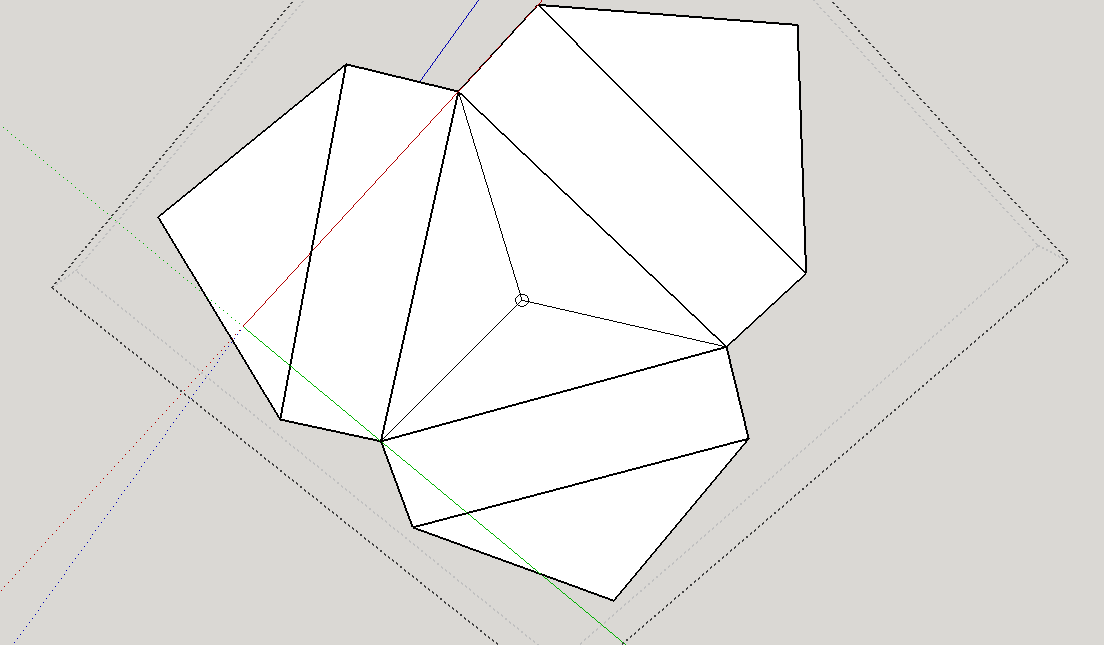
\includegraphics[scale=0.25]{starUnfolding/h3SpanningOne.png}
\end{figure}

\begin{figure}[h]
\caption{$H_3$ edge unfolded and with shortest paths drawn to all vertices. }
\centering
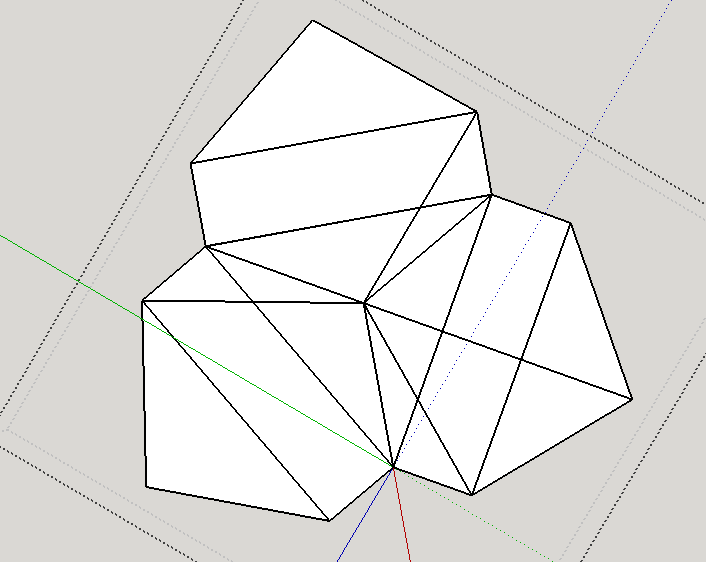
\includegraphics[scale=0.25]{starUnfolding/h3Spanning.png}
\end{figure}


%\begin{figure}[h]
%\centering
%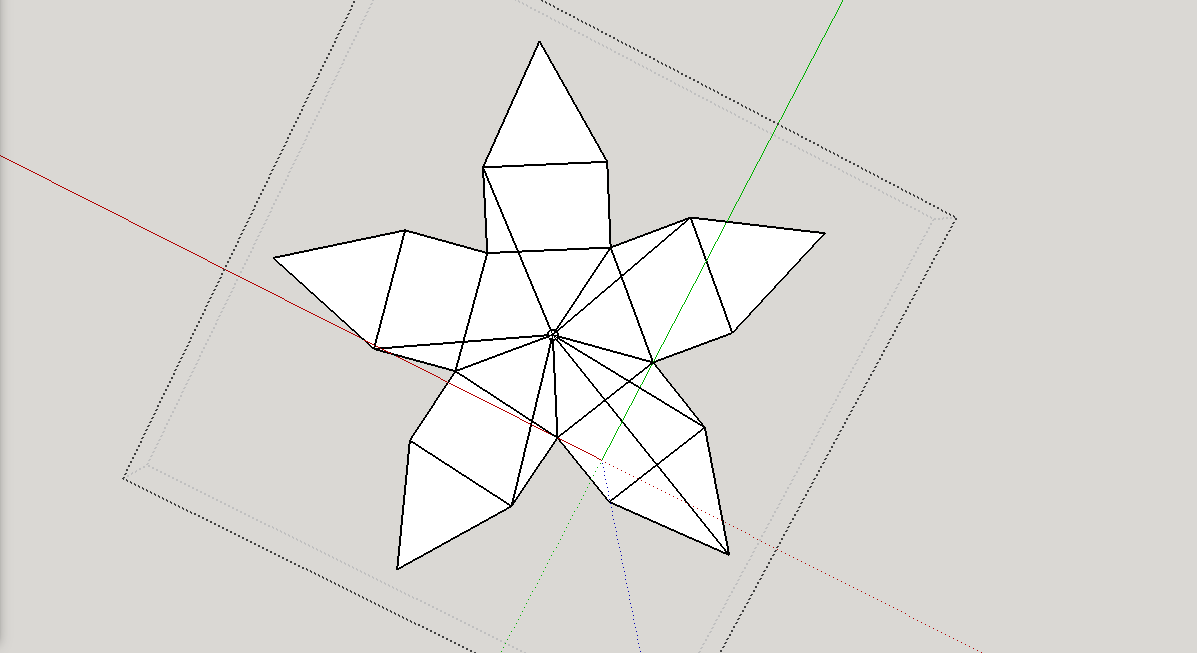
\includegraphics[scale=0.15]{starUnfolding/h5Spanning.png}
%\end{figure}

%\begin{figure}[h]
%\centering
%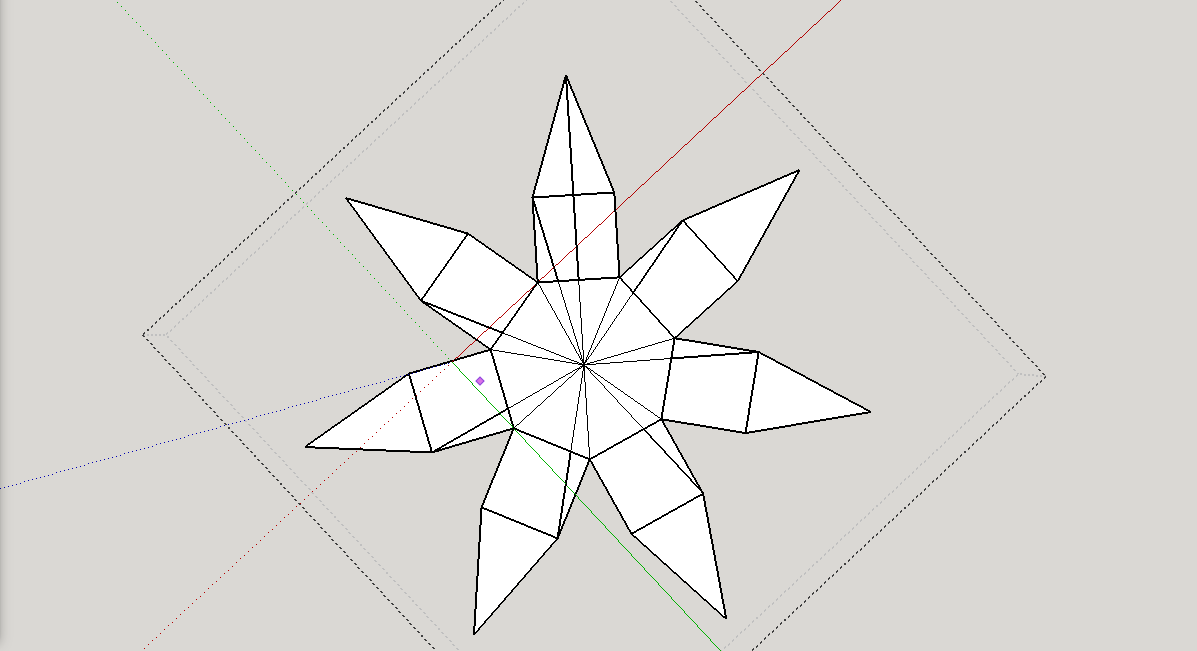
\includegraphics[scale=0.15]{starUnfolding/h7Spanning.png}
%\end{figure}

%\begin{figure}[h]
%\centering
%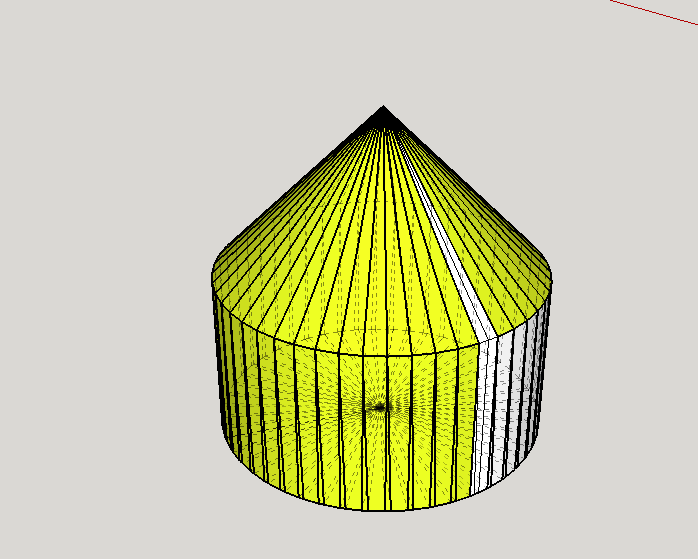
\includegraphics[scale=0.15]{starUnfolding/h50Spanning.png}
%\end{figure}

\section{Star Unfolding}
%\begin{figure}[h]
%\caption{$H_4$ edge unfolded and with shortest paths drawn to all vertices.}
%\centering
%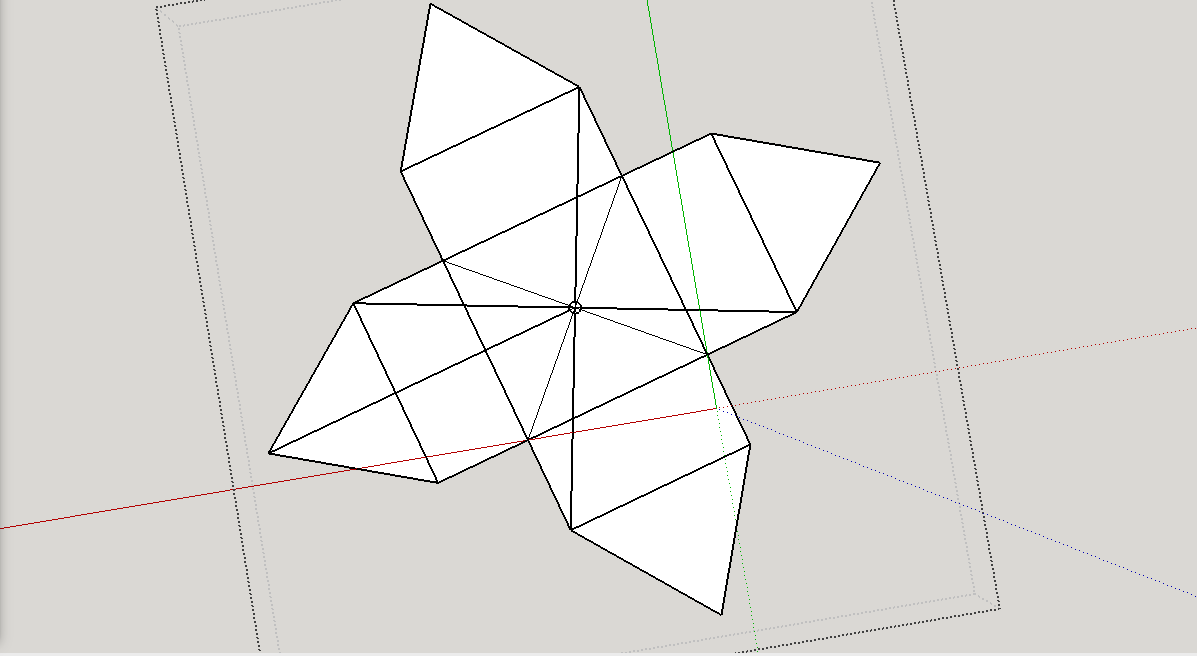
\includegraphics[scale=0.25]{starUnfolding/h4Spanning.png}
%\end{figure}
Now that cutting trees for each of the 5 cases have been defined, the UPN of each polyhedron can be found by defining a star unfolding for each polyhedra.

A star unfolding is defined as the mapping \cite{GFALOP:1} of the cutting tree $T$ onto a plane, where every edge of $T$ is mapped to two edges on the UPN, and each node, except the source point, is mapped to two vertices. This can be 
After finding the minimum spanning trees for the house-shaped polyhedra, I refolded them back into their polyhedral forms. Notice that due to the new edges introduced by the cutting tree, there are new, distinct faces that were formed from the original faces by being split by the cutting tree. The faces are  colored to show how each one was split.
\begin{figure}[h]
\centering
\caption{$H_3$ refolded and colored.}
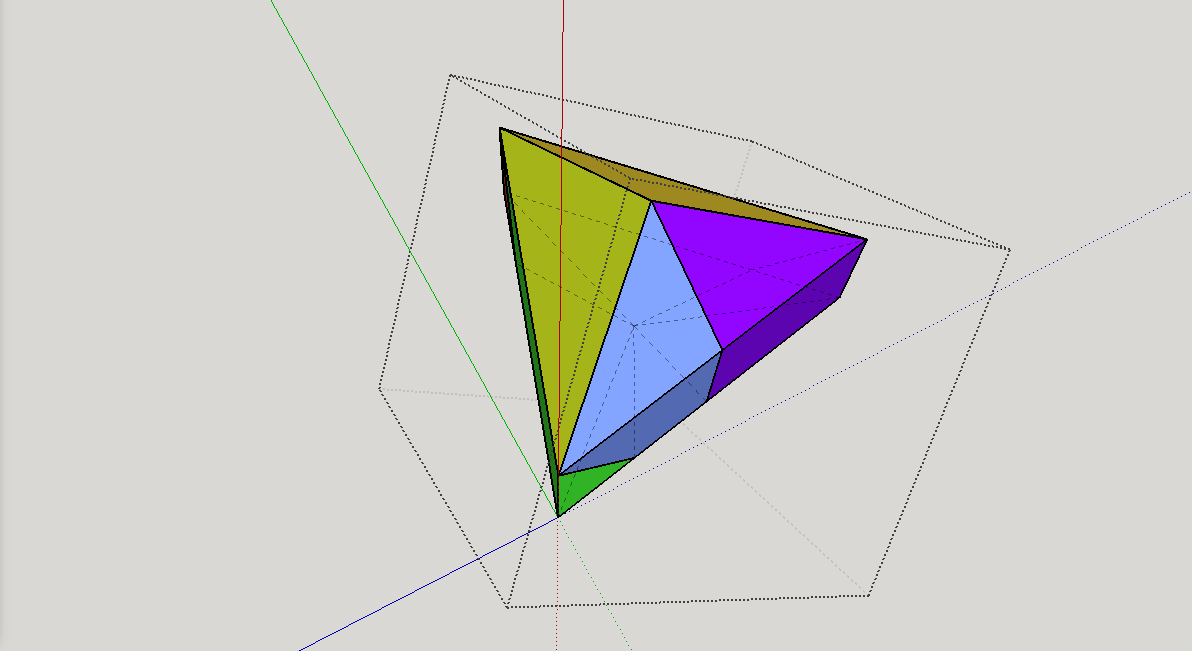
\includegraphics[scale=0.15]{finalUNP/h3ColorTop.png}
\end{figure}
Notice how there are some faces that weren't touched by the cutting tree. These faces, colored yellow, are what Alexandrov \cite{ALEXANDROV} defined as the core of the star unfolding. They remain unsplit, and are in the centre of the final UPN.
 The new edges defined by the cutting tree, once unfolded, would each define two edges in the UPN. Unfolding the polyhedron would also yield multiple images of the nodes in the cutting tree, as the star unfolding yields a double of the number of vertices 
 
We may now begin unfolding the polyhedra flat along its edges to define a new polygon using the edges and nodes of the cutting tree. 
Each face was rotated along an edge that wasn't a cut, and doesn't belong to $T$, until all the faces are coplanar. Once this is done, the UPN will have been successfully defined.

\begin{figure}[h]
\label{STARS}
\underline{Star Unfoldings}
\centering
\begin{subfigure}[t]{0.25\textwidth}
\caption{Star Unfolding of $H_3$}
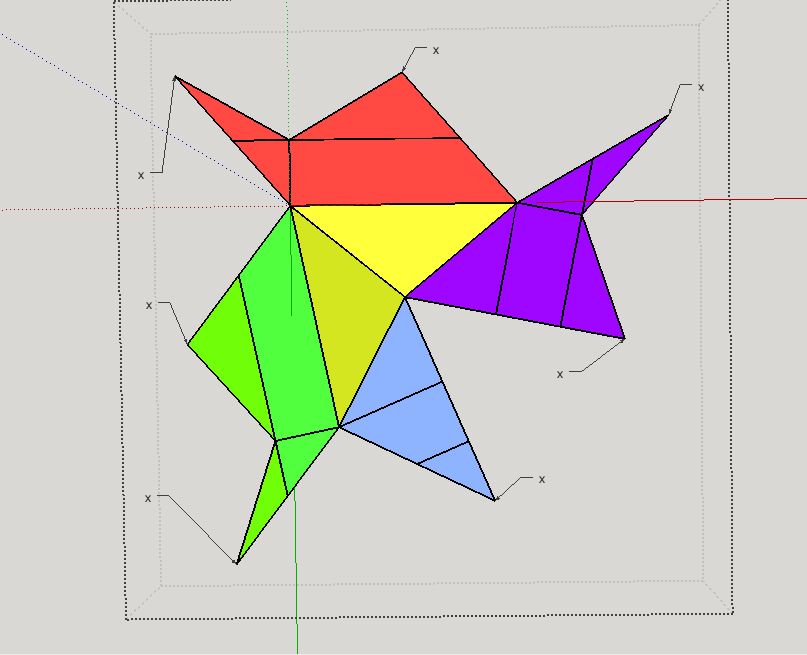
\includegraphics[scale=0.15]{finalUNP/h3UNP.png}
\end{subfigure}%
%
\begin{subfigure}[t]{0.25\textwidth}
\caption{Star Unfolding of $H_4$ }
\centering
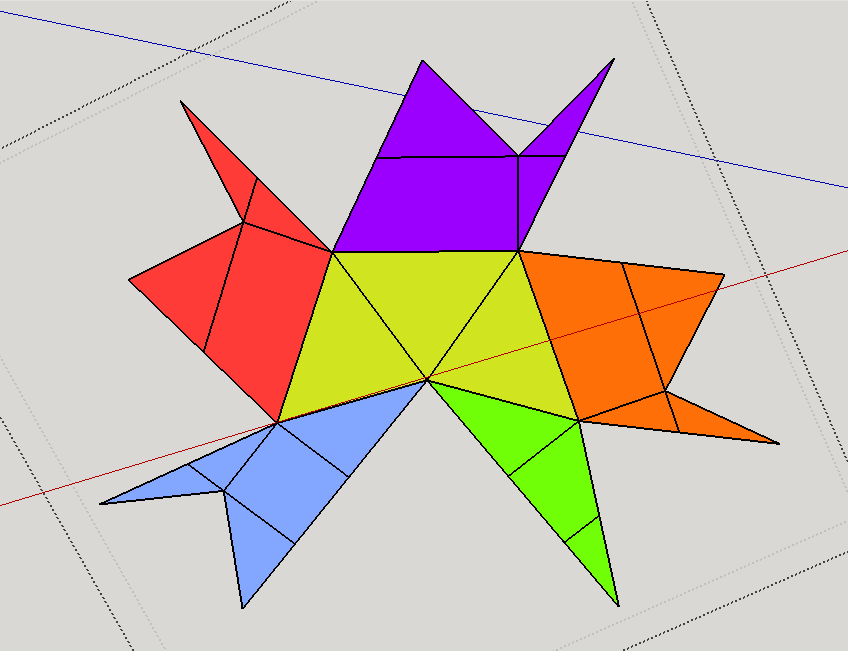
\includegraphics[scale=0.15]{finalUNP/h4UNP.png}
\end{subfigure}%
%
\begin{subfigure}[t]{0.25\textwidth}
\caption{Star Unfolding of $H_5$ }
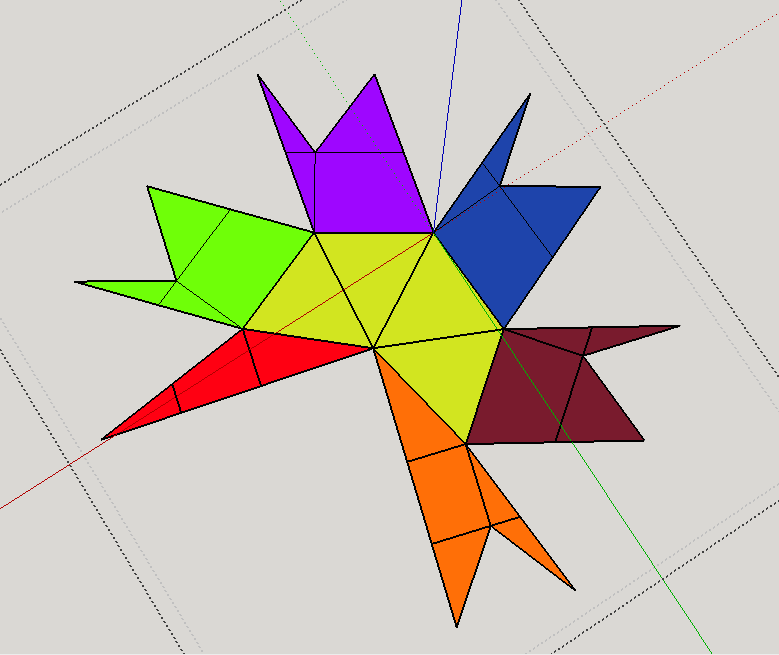
\includegraphics[scale=0.15]{finalUNP/h5UNP.png}
\end{subfigure}%
\begin{subfigure}[t]{0.25\textwidth}
\caption{Star Unfolding of $H_6$ }
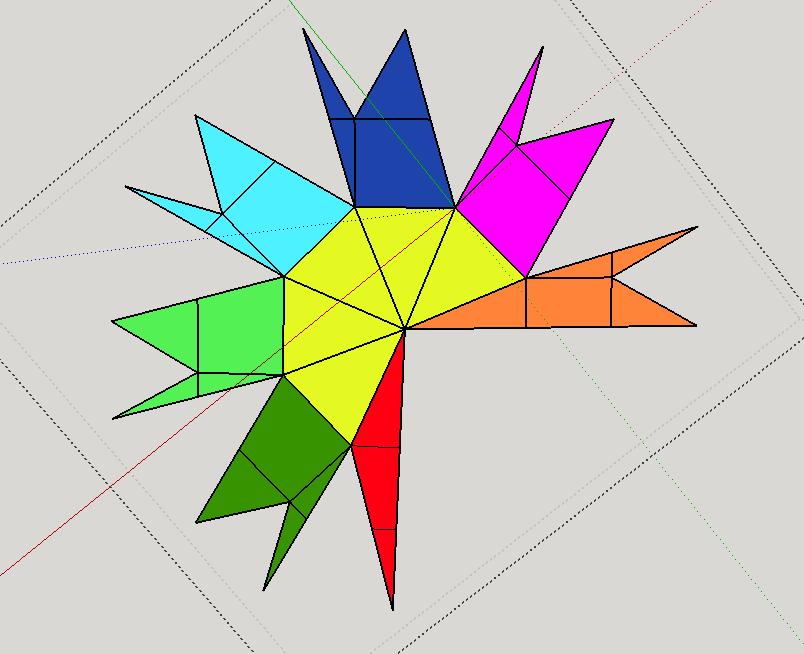
\includegraphics[scale=0.15]{finalUNP/h6UNP.png}
\end{subfigure}
\end{figure}%

\begin{figure}[h]
\caption{Star Unfolding of $H_{50}$ (uncolored except for the core)}
\centering
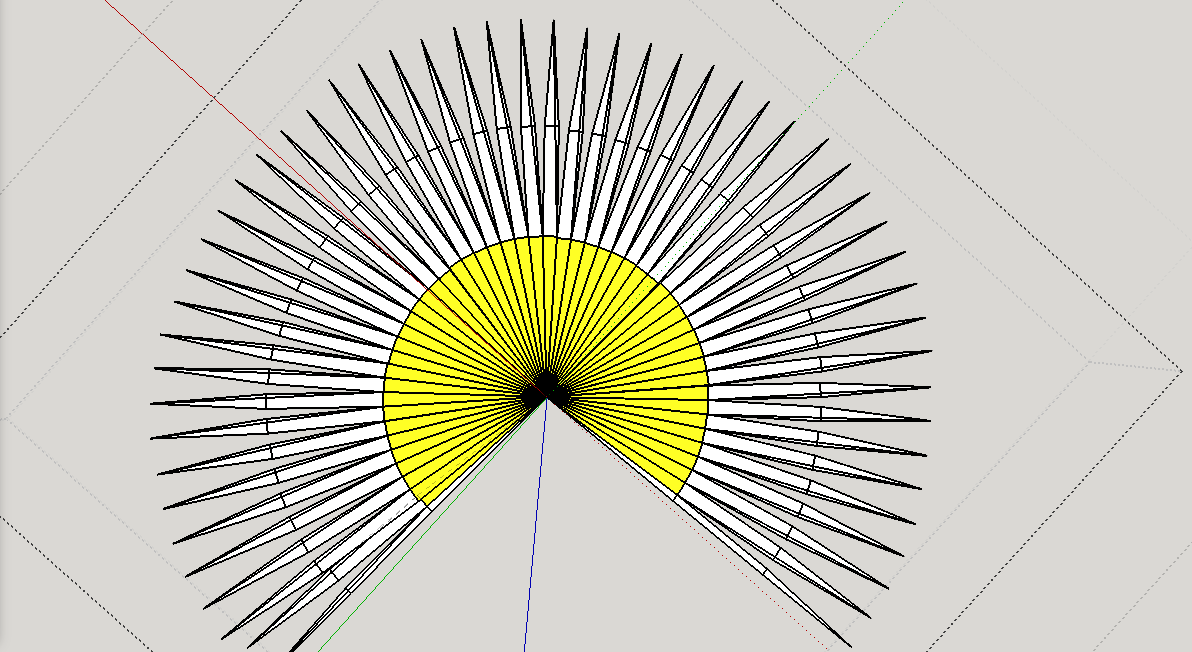
\includegraphics[scale=0.3]{finalUNP/h50UNP.png}
\end{figure}
\newpage


\section{Cut Locus}

	Using the star unfoldings generated in the last section, a Voronoi diagram was drawn from the vertices of each UPN. The diagrams were drawn by using a Sketchup plugin developed by the Sketchup users community. However, this formed a boundary that was bigger than the boundary of the UPN. The outline of the UPN was then drawn onto the Voronoi diagrams (blue highlighting) to constrain them to just the surface bound by the star unfoldings. 
\begin{figure}[h]
\centering
	\begin{subfigure}[t]{0.4\textwidth}
	\caption{Voronoi Diagram of $H_3$}
	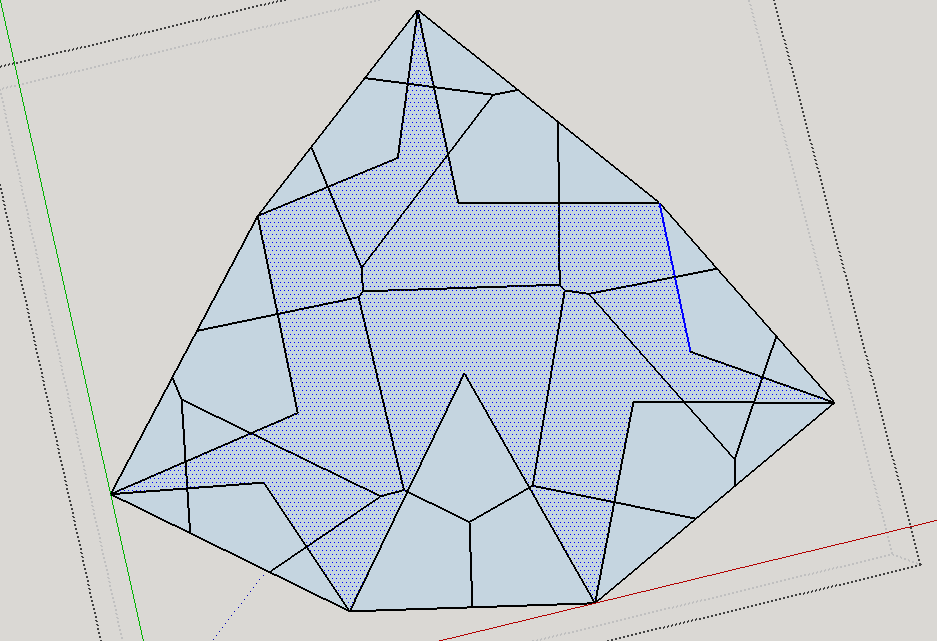
\includegraphics[scale=0.17]{vDiags/h3Voronoi.png}
	\end{subfigure}
	\begin{subfigure}[t]{0.4\textwidth}
	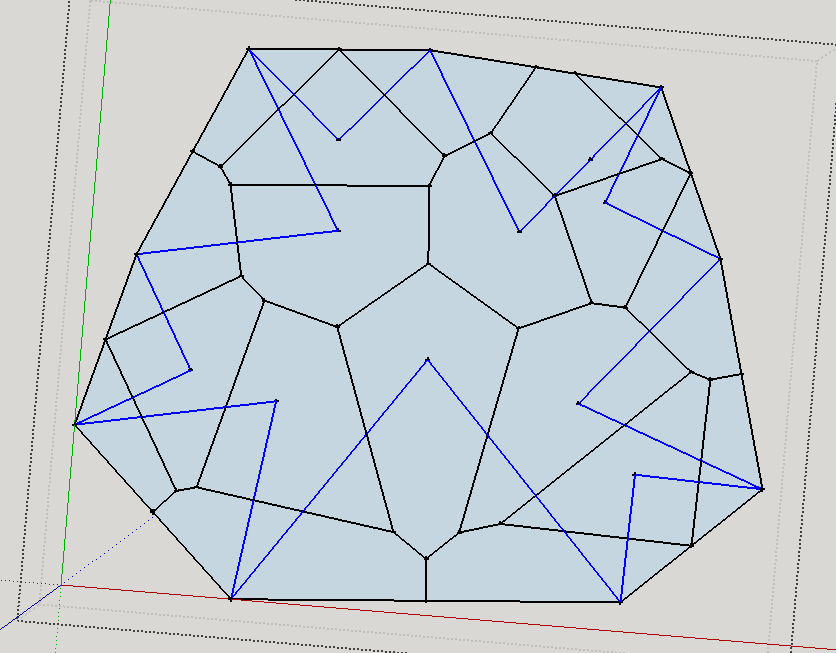
\includegraphics[scale=0.17]{vDiags/h4Voronoi}
	\caption{Voronoi Diagram of $H_4$}
	\end{subfigure}
\end{figure}	
\begin{figure}[h]
\centering
	\begin{subfigure}[t]{0.4\textwidth}
	\caption{Voronoi Diagram of $H_5$}
	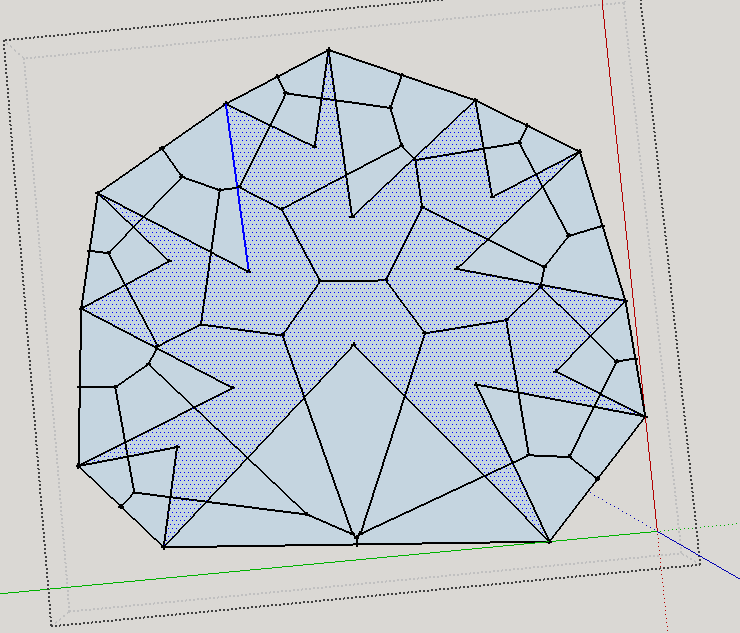
\includegraphics[scale=0.2]{vDiags/h5Voronoi.png}
	\end{subfigure}
	
	\begin{subfigure}[t]{0.4\textwidth}
	\caption{Voronoi Diagram of $H_6$}
	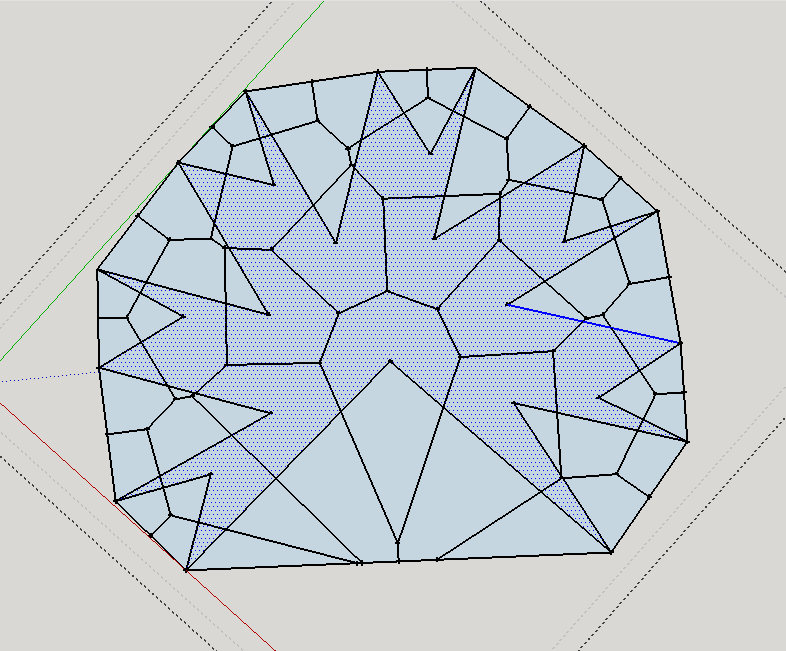
\includegraphics[scale=0.2]{vDiags/h6Voronoi.png}
	\end{subfigure}
	
\end{figure}
\newpage
\section{Patterns}
Across the star unfoldings and voronoi diagrams of different house-shaped polyhedra, there were several repeating shapes. Parts of the star unfoldings that weren?t the core seem to be made from three distinct shapes. The most common shape is the shape that attaches itself to the outsides of the star unfolding cores, called the main spines, or m-spines. These would be the purple, red and orange shapes in the star unfolding of $H_4$. For every additional side added to the base of a house-shaped polyhedron, there is an additional m-spine added to the star unfolding, and then they are collectively shrunk. In general, for a polyhedron $H_n$, there are $n-1$ m-spines and 1 a-spine and 1 b-spine. The shrinking property is apparent in the star unfolding of $H_{50}$, where the m-spines become much thinner than those in $H_3$. This can be attributed to the fact that as $n$ increases, which causes the number of edges on the base of $H_n$ to also increase, the edge length shrinks. 

Two other shapes that are common across the star unfoldings are the spines which are attached to the ends of the cores in the star unfoldings. In the star unfolding of $H_{4}$, they are the baby blue and green colored faces. Let them be called a-spines and b-spines respectively. Unlike m-spines, they only get smaller as the edge length of the base decreases. They come from a lateral face of the pyramid being split in two by an edge of the cutting tree which extended to the apex of the pyramid, which generates a two-pointed b-spine and a thinner a-spine.

The cores and the m-spines of the star unfoldings produce Voronoi edges that meet in a vertex. The number of these Voronoi vertices also increases with $n$, with $H_n$ also producing $n-1$ Voronoi vertices within the regions of the cores and the m-spines. 

\section{Conclusion}
As $n$ approaches infinity, the inner boundary of the cores of the star unfoldings of $H_n$ approaches a circle, and the cut locus within the cores of the star unfolding approach the medial axis in within that region.
It is difficult to say what occurs within the regions enclosed by the a, m, and b spines. However, seeing that the edge lengths of the base of $H_n$ approach zero, it can be conjectured that the spines will disappear entirely, leaving just the cores and the Voronoi edges enclosed within them.

\textbf{Word Count}: 3445

\newpage

%%Bibliography
\bibliography{EEBibliography}
\bibliographystyle{ieeetr}

\end{document}